\subsection{Photo-multipliers dividers}

In the original readout electronics the LTCC single output from each PMT was amplified by a factor of 10
and then split in two to feed the ADC and TDC boards. This amplification and splitting was performed
by a dedicated electronic module (UVA 132) \cite{Adams:2001kk}. This was replaced by a pulse amplifier entirely powered by
the current flowing through the base voltage divider, developed in 2002 at Jefferson Lab \cite{Popov:2003mj}.
The new electronics provided a factor of 10 PMT signal boost while preserving the fast PMT pulse shape. It also significantly improved signal amplitude and
signal to noise ratio: the high voltage needed to detect the single photo-electron signal (SPE) was reduced from in average by 360 V, see \F{pmtHVImprovement}.

\begin{figure}
	\centering
	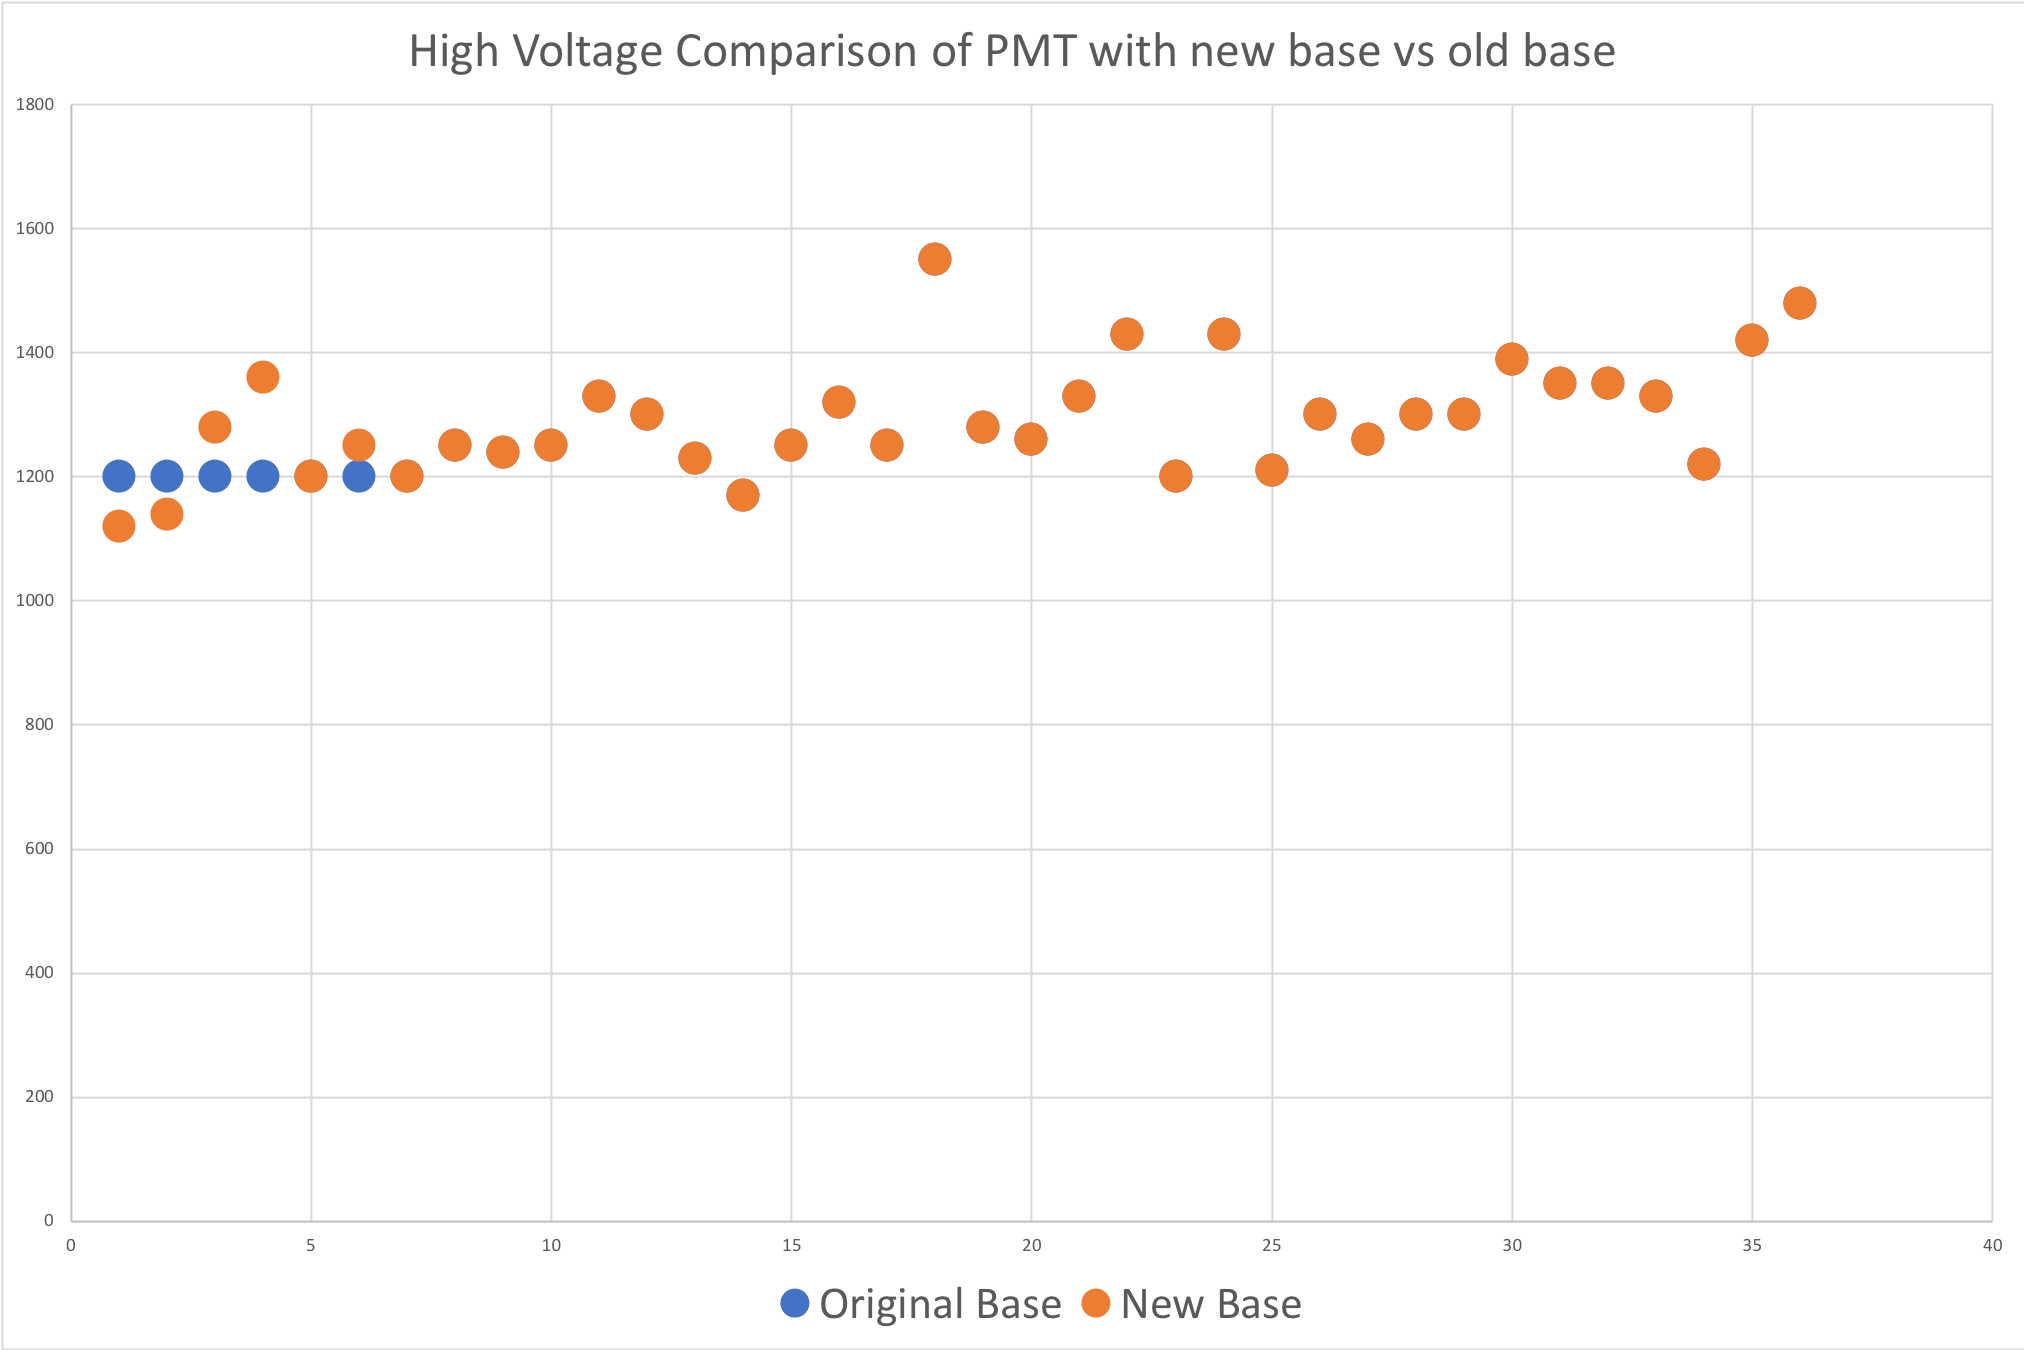
\includegraphics[width=0.95\columnwidth,keepaspectratio]{img/pmtHVImprovement.png}
	\caption{Comparison of the PMT high voltages in sector 5 gain-matched to provide a SPE peak at about ADC channel 200.
            The PMTs with the modified bases produce the same response function of the original base but at an average voltage 360 HV less (1666 V vs 1292 V).}
	\label{fig:pmtHVImprovement}
\end{figure}

The design was adapted to use the LTCC XP4500B base and a prototype, shown in \F{pmtWithDivider}, was built to provide a x10
amplification and a split signal directly from the PMT base.

\begin{figure}
	\centering
	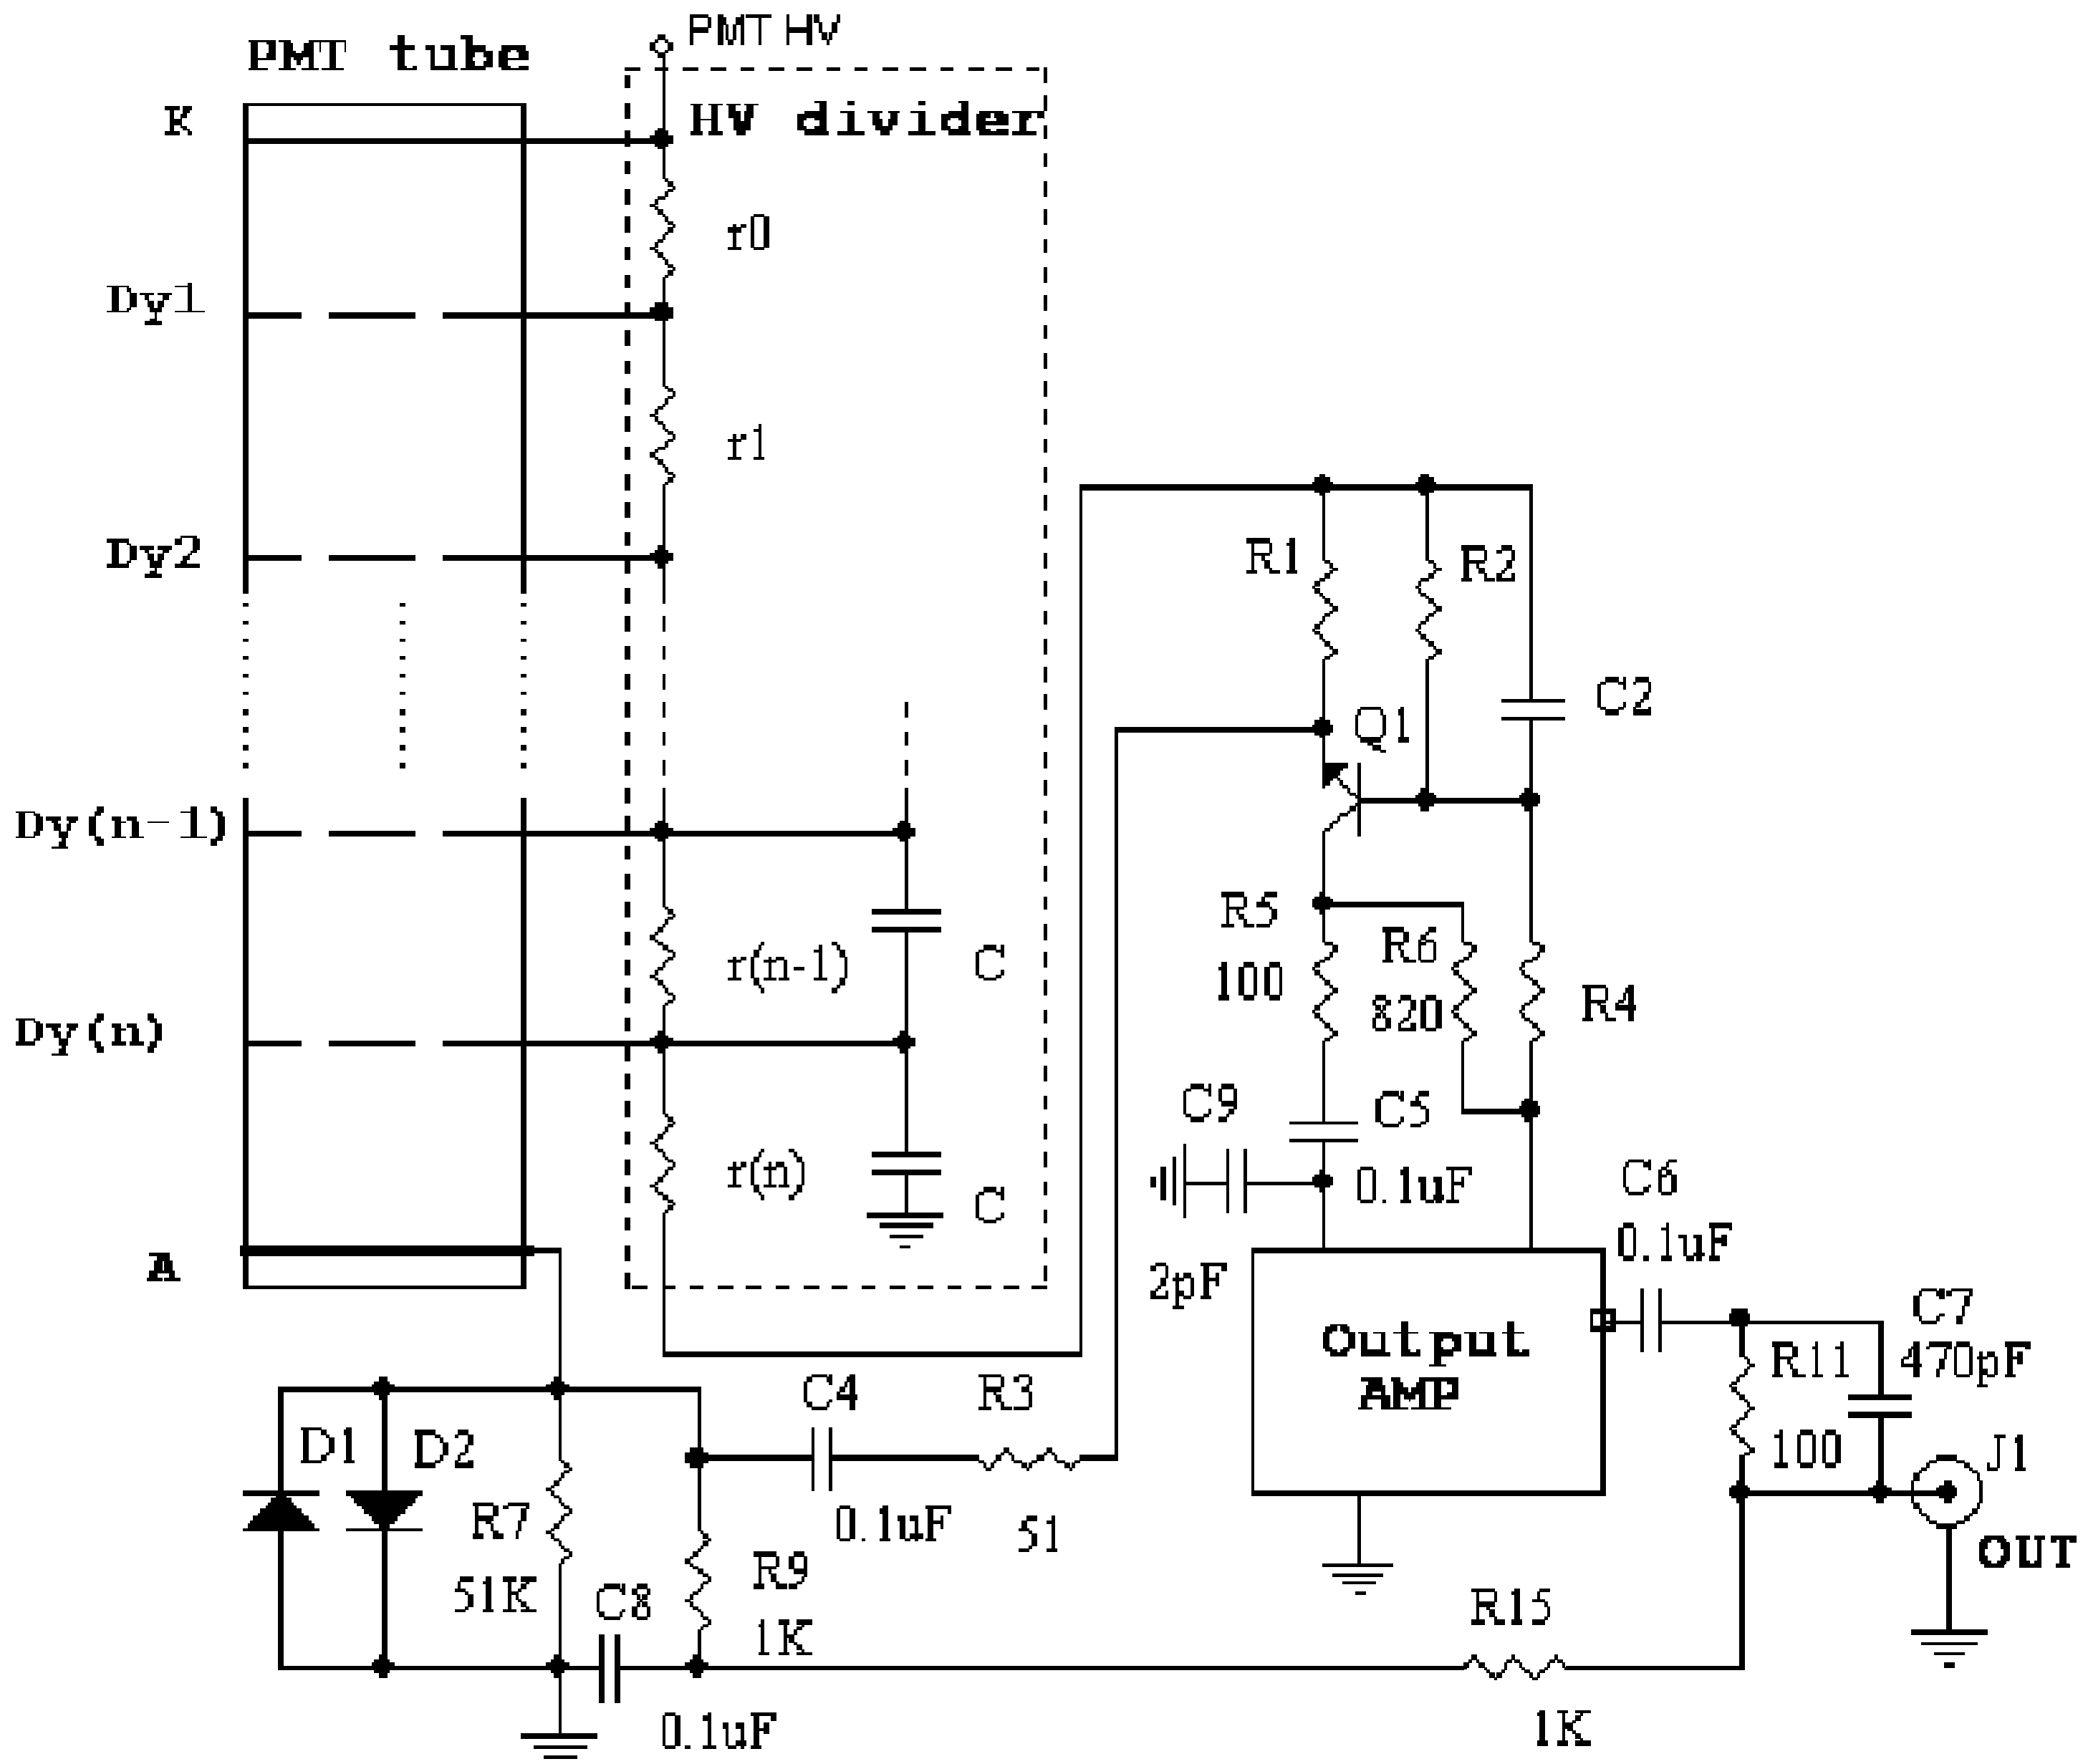
\includegraphics[width=0.95\columnwidth,keepaspectratio]{img/dividerSchematic.png}
	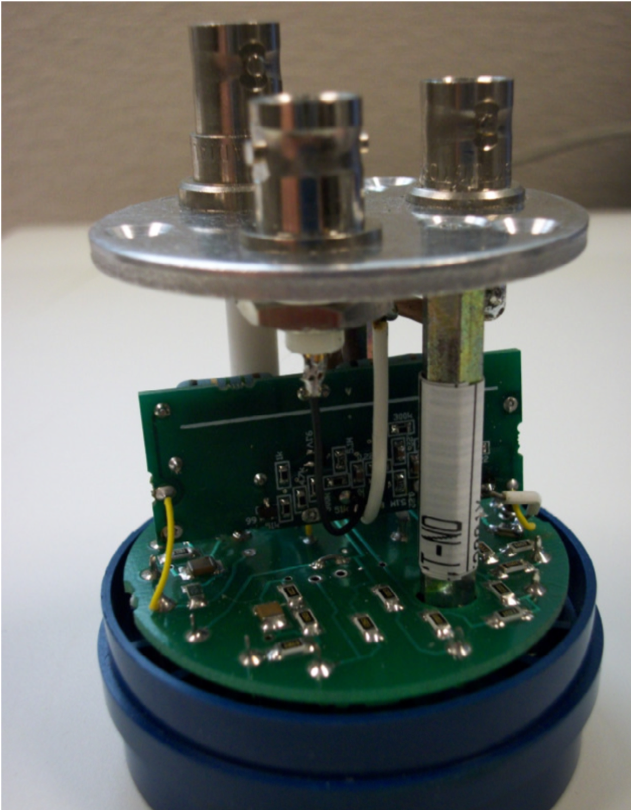
\includegraphics[width=0.95\columnwidth,keepaspectratio]{img/pmtWithDivider.png}
	\caption{Top: schematic of the board, shown as a resistor chain for simplicity. The amplifier, designed to operate at current from 0.7 to 1.5 mA,
            provides amplification in the first stage using a common base amplifier, made on a fast NPN transistor NE68033 by California Eastern Laboratories.
            In the output stage a PNP-NPN transistors is used.
            Bottom: the prototype module installed in the XP4500B PMT base.
            The bottom of the base has been modified to contain the HV SHV input and two output signals. }
	\label{fig:pmtWithDivider}
\end{figure}

In \F{dividerTests} (top) a comparison of the two signals shows the similarity between the two outputs.
During testing of the modified PMT bases, the output has been processed by a Flash ADC and acquired with a data
acquisition software using the PMT itself as trigger.
The corresponding SPE spectrum has been analyzed. The shape of the SPE signal is very similar to the original signal
coming from the external dedicated splitter and amplifier through the ADC electronics, see  \F{dividerTests} (bottom).

\begin{figure}
	\centering
	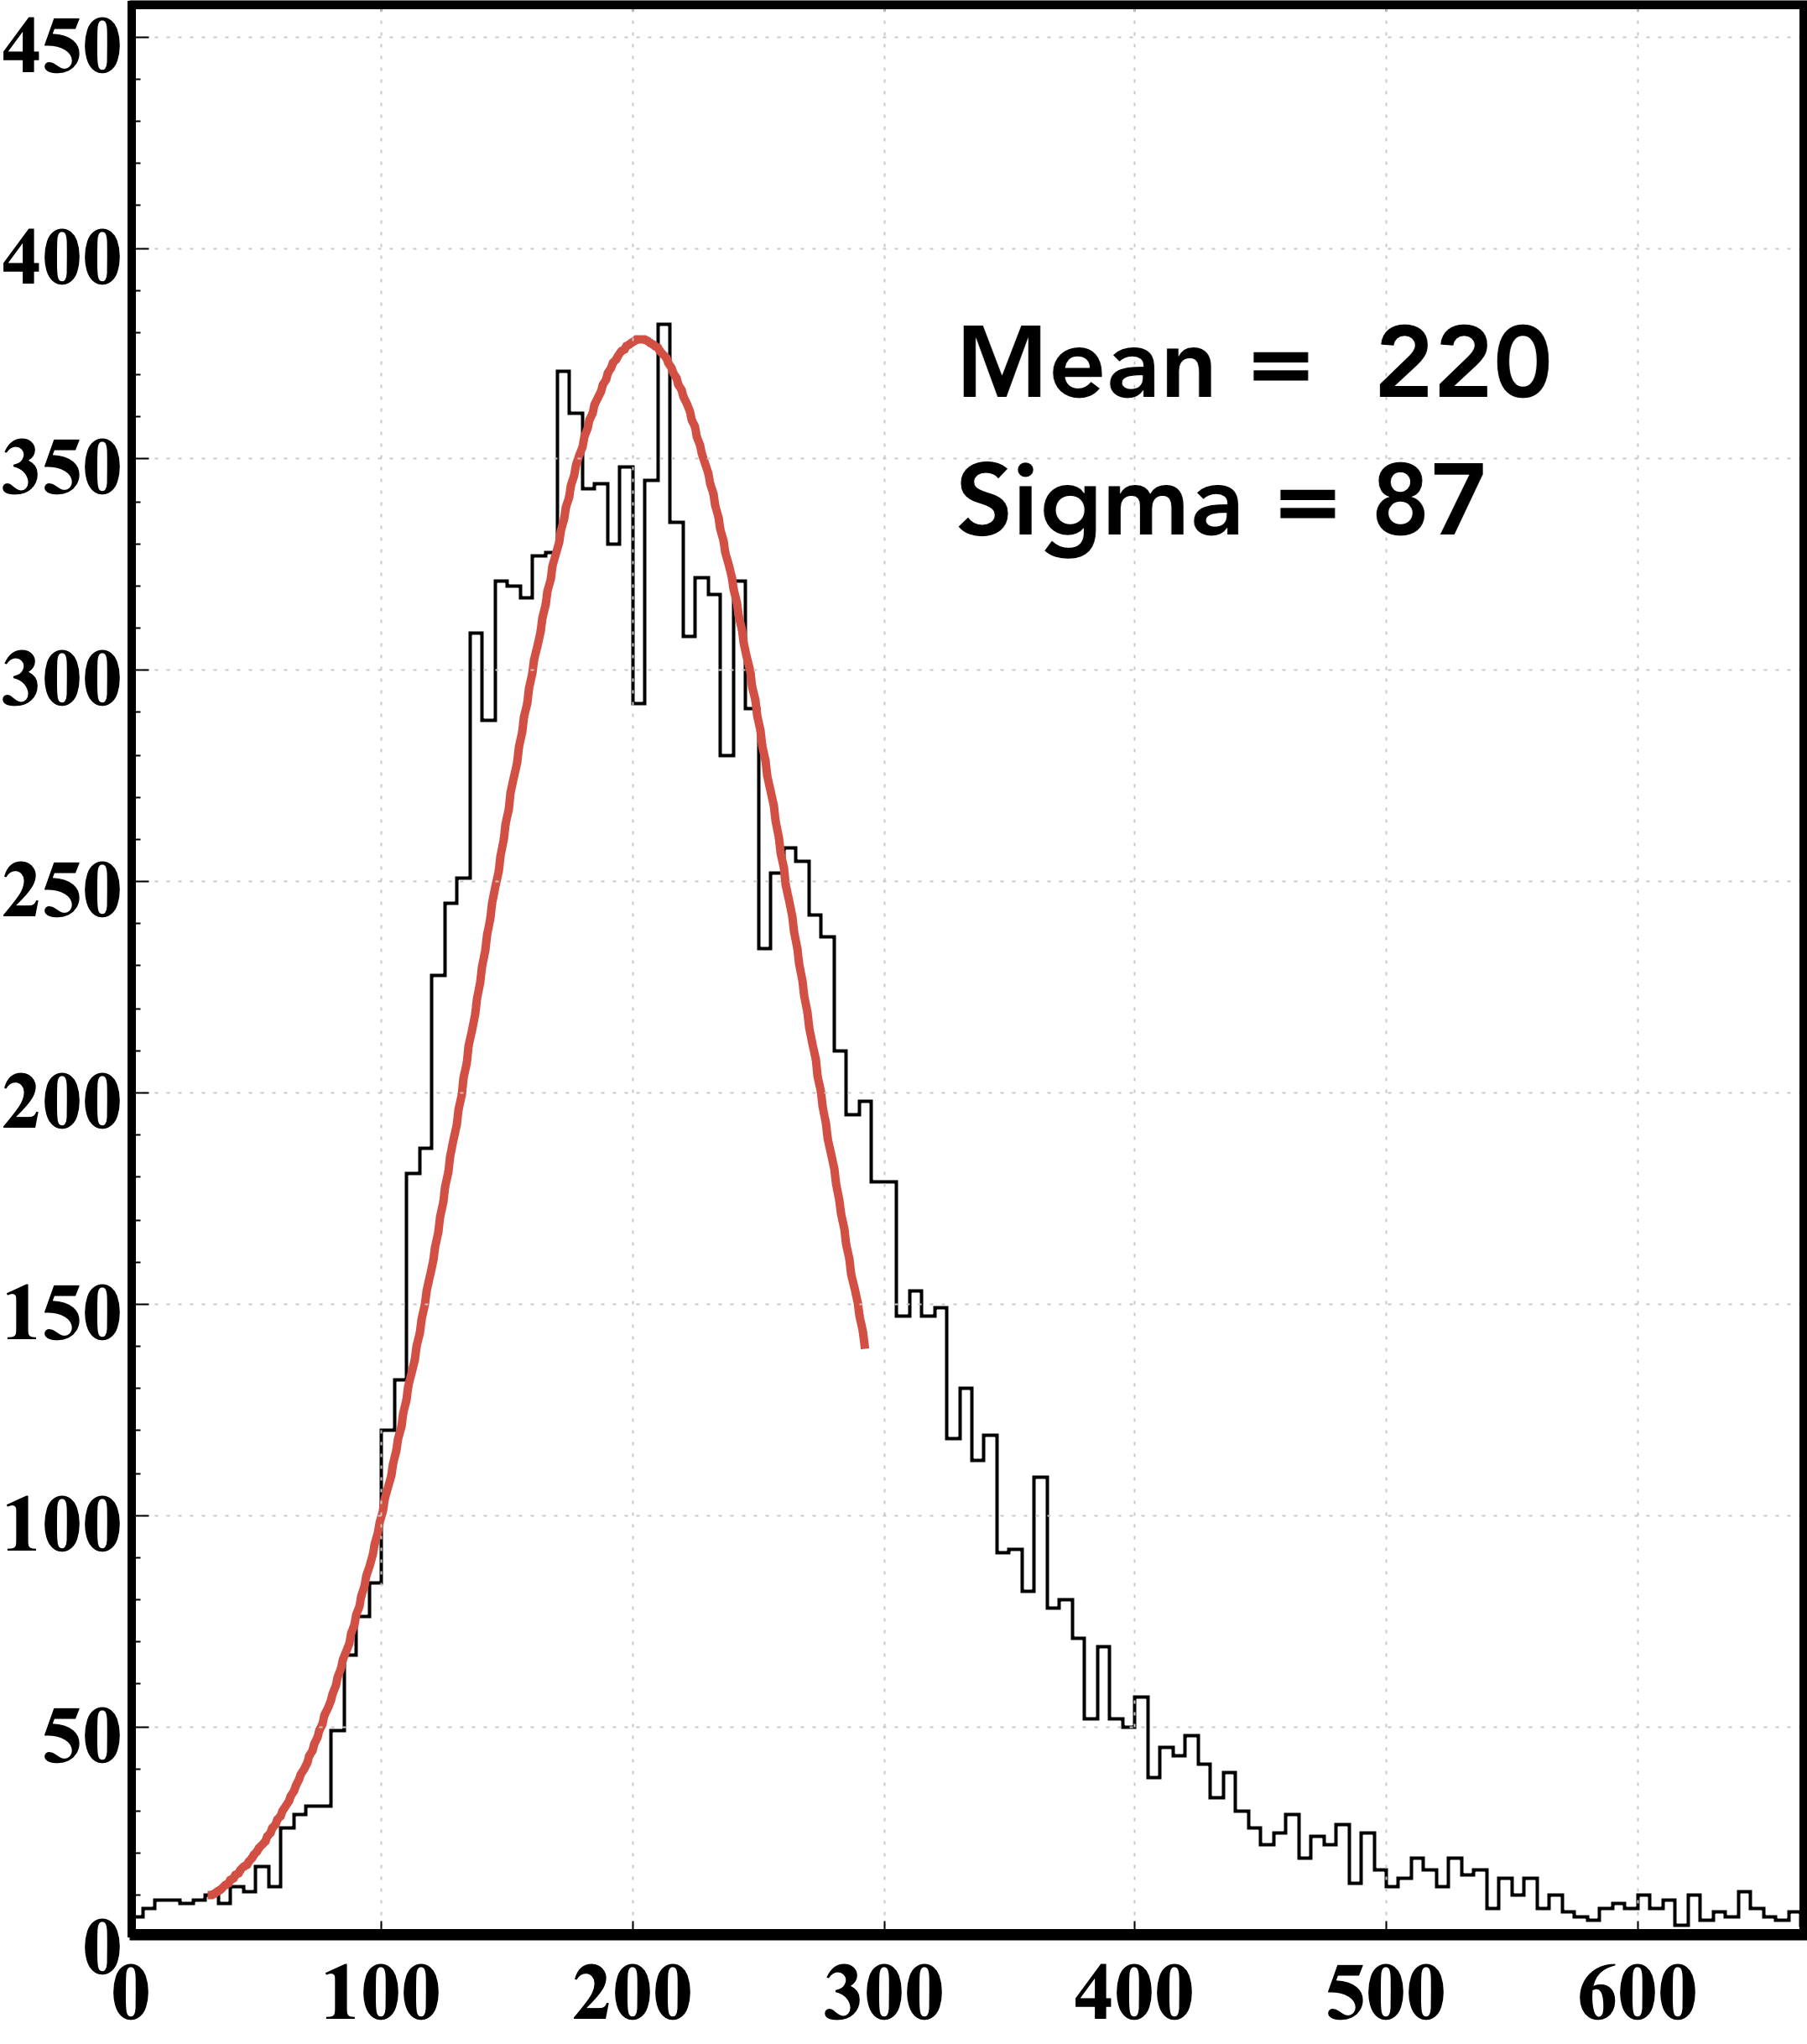
\includegraphics[width=0.95\columnwidth,keepaspectratio]{img/fadcOutput.png}
	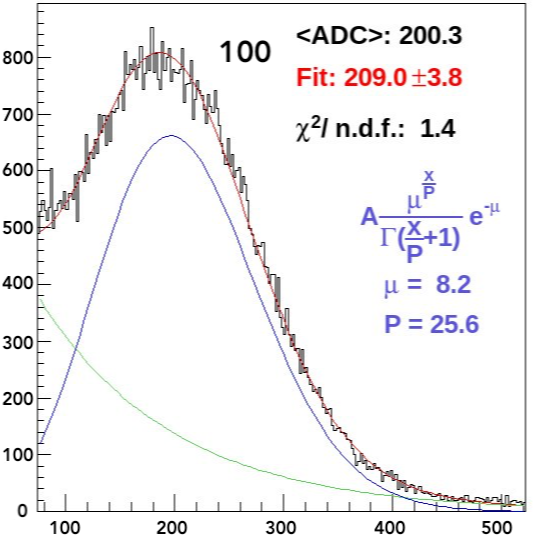
\includegraphics[width=0.97\columnwidth,keepaspectratio]{img/cc_signal.png}
	\caption{The single photo-electron FADC spectrum of one of the PMTs with the modified base (top) compared with the original ADC output in the
            configuration of a dedicated external splitter and amplifier (bottom). }
	\label{fig:dividerTests}
\end{figure}

180 bases were assembled at Jefferson Lab and installed on the PMT dividers. Both signals from all the modified bases were tested.
The response of the PMTs, amplified by a factor of 10, was verified to be identical to the original output.


